\documentclass[]{ximera}
%handout:  for handout version with no solutions or instructor notes
%handout,instructornotes:  for instructor version with just problems and notes, no solutions
%noinstructornotes:  shows only problem and solutions

%% handout
%% space
%% newpage
%% numbers
%% nooutcomes

%I added the commands here so that I would't have to keep looking them up
%\newcommand{\RR}{\mathbb R}
%\renewcommand{\d}{\,d}
%\newcommand{\dd}[2][]{\frac{d #1}{d #2}}
%\renewcommand{\l}{\ell}
%\newcommand{\ddx}{\frac{d}{dx}}
%\everymath{\displaystyle}
%\newcommand{\dfn}{\textbf}
%\newcommand{\eval}[1]{\bigg[ #1 \bigg]}

%\begin{image}
%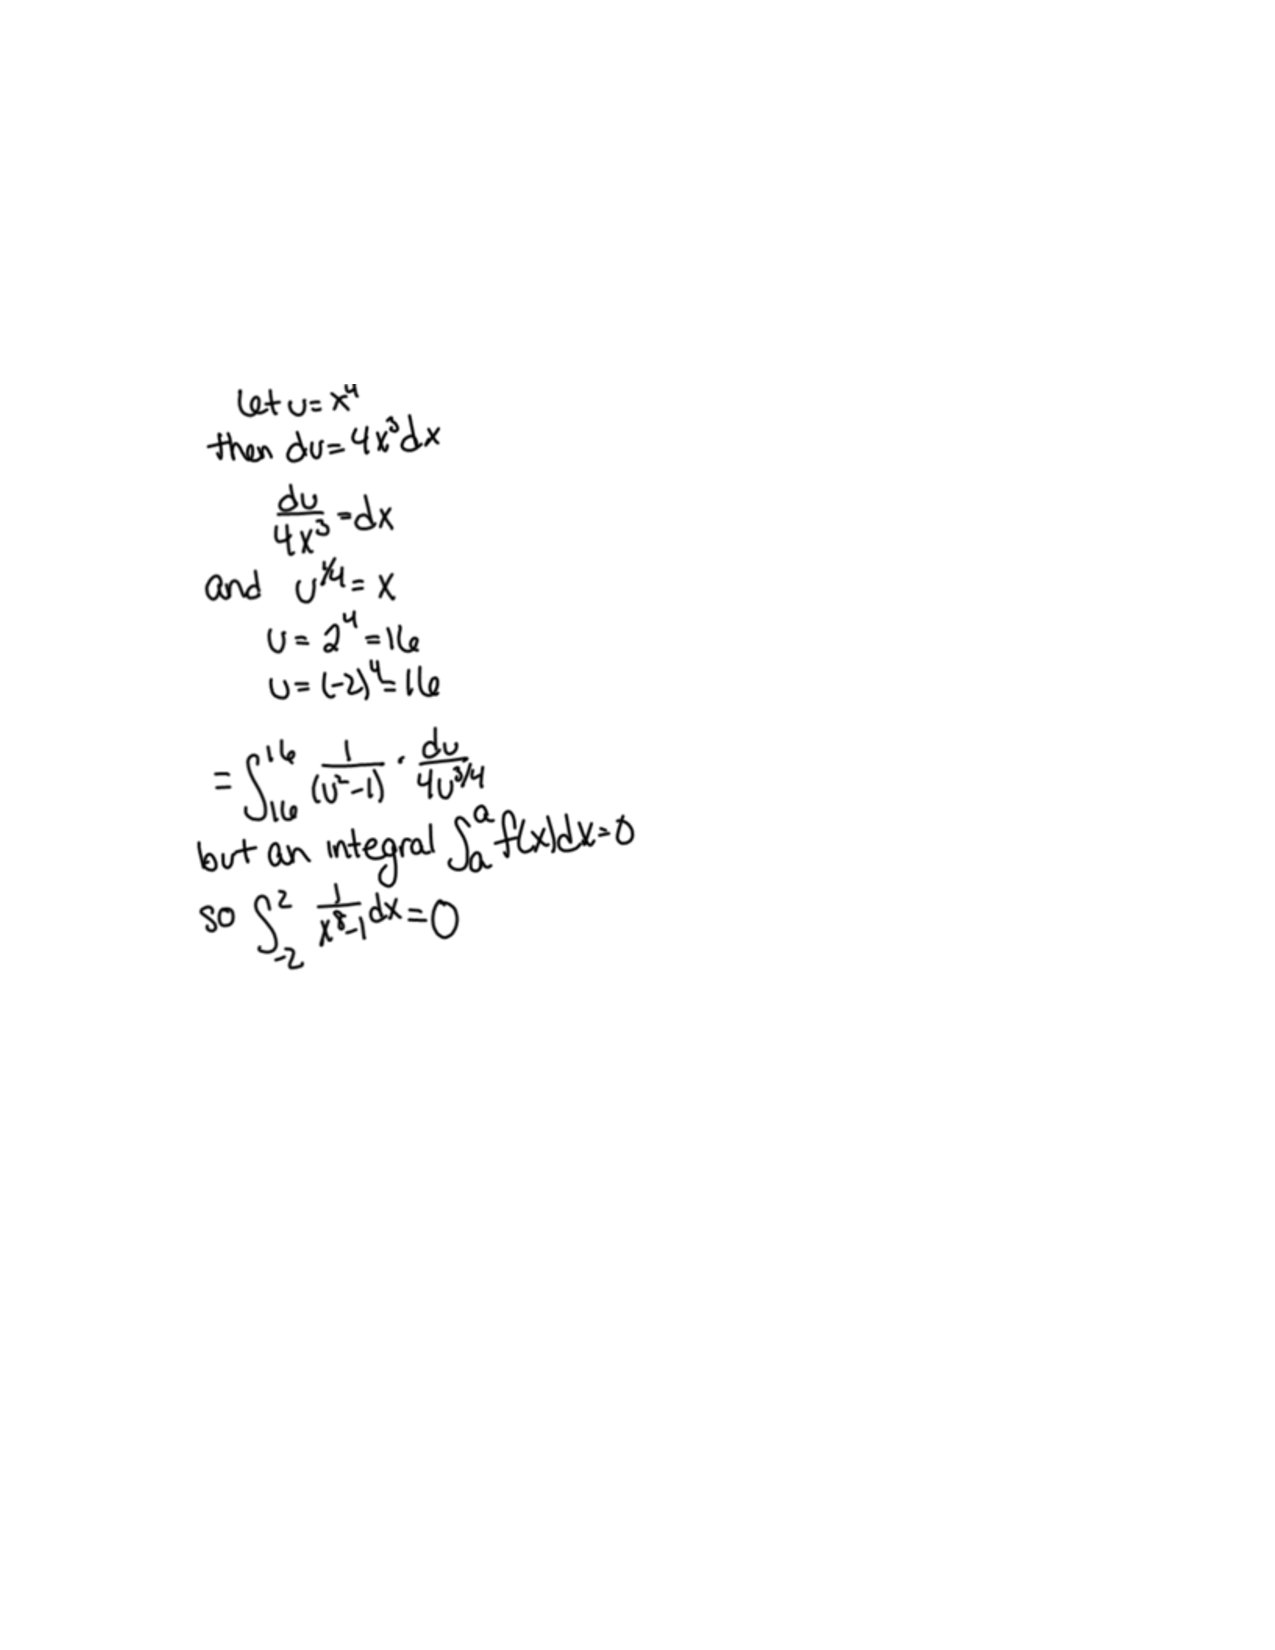
\includegraphics[trim= 170 420 250 180]{Figure1.pdf}
%\end{image}

%add a ``.'' below when used in a specific directory.
\newcommand{\RR}{\mathbb R}
\renewcommand{\d}{\,d}
\newcommand{\dd}[2][]{\frac{d #1}{d #2}}
\renewcommand{\l}{\ell}
\newcommand{\ddx}{\frac{d}{dx}}
\newcommand{\dfn}{\textbf}
\newcommand{\eval}[1]{\bigg[ #1 \bigg]}

\usepackage{multicol}

\renewenvironment{freeResponse}{
\ifhandout\setbox0\vbox\bgroup\else
\begin{trivlist}\item[\hskip \labelsep\bfseries Solution:\hspace{2ex}]
\fi}
{\ifhandout\egroup\else
\end{trivlist}
\fi} %% we can turn off input when making a master document

\title{Lines and curves in space}  

\begin{document}
\begin{abstract}		\end{abstract}
\maketitle



\section{Warm up:}
Find a vector-valued function for the line segment connecting the points $P = (-3,7,6)$ and $Q = (5,-4,7)$ in such a way that the value at $t=0$ is $P$ and the value at $t=1$ is $Q$.  
Also, find the point two-thirds of the way from $P$ to $Q$.
	\begin{freeResponse}
	The line segment $\vec{r}(t)$ from $P$ to $Q$ is 
		\begin{align*}
		\vec{r}(t) &= (1-t)P + tQ  \\
		&= (1-t) \langle -3,7,6 \rangle + t \langle 5,-4,7 \rangle  \\
		&= \boxed{\langle -3 + 8t, 7 - 11t, 6 + t \rangle \quad \text{for }0 \leq t \leq 1}.
		\end{align*}
	The point two-thirds of the way from $P$ to $Q$ is
		\begin{align*}
		\vec{r} \left( \frac{2}{3} \right)
		&= \left\langle -3 + 8 \left( \frac{2}{3} \right), 7 - 11\left( \frac{2}{3} \right), 6 + \frac{2}{3} \right\rangle  \\
		&= \boxed{\left\langle \frac{7}{3} , - \frac{1}{3}, \frac{20}{3} \right\rangle}
		\end{align*}
	\end{freeResponse}
	
\begin{instructorNotes}
%There were no instructor notes for this handout.
\end{instructorNotes}







\section{Group work:}



%problem 1
\begin{problem}
Find a vector-valued function for the line through the point $(1,-2,3)$ that is perpendicular to the lines
	\[
	\vec{r}_1(t) = \langle 7,8,-2 \rangle + t \langle 3,5,7 \rangle 
	\quad \text{and} \quad 
	\vec{r}_2(s) = \langle 4,-3,-7 \rangle + s \langle 4,9,-1 \rangle
	\]
	\begin{freeResponse}
	Let $\vec{v}_1 = \langle 3,5,7 \rangle$ and $\vec{v}_2 = \langle 4,9,-1 \rangle$.
	Then $\vec{v}_1$ is parallel to the line $\vec{r}_1$, and similarly for $\vec{v}_2$ and $\vec{r}_2$.  
	So a vector perpendicular to both of the lines $\vec{r}_1$ and $\vec{r}_2$ is
		\begin{align*}
		\vec{n} = \vec{v}_1 \times \vec{v}_2  
		&= \begin{vmatrix}
		\hat{\imath}	&	\hat{\jmath}	&	\hat{k}	\\
		3		&	5		&	7		\\
		4		&	9		&	-1		\\
		\end{vmatrix}  \\
		&= (-5-63)\hat{\imath} - (-3-28)\hat{\jmath} + (27-20)\hat{k}  \\
		&= \langle -68, 31, 7 \rangle.
		\end{align*}
	So the equation of the line through $(1,-2,3)$ and perpendicular to both $\vec{r}_1$ and $\vec{r}_2$ is
		\begin{align*}
		\vec{r}_3(t) &= \langle 1,-2,3 \rangle + t \langle -68,31,7 \rangle  \\
		&= \boxed{\langle 1-68t,-2+31t,3+7t \rangle \quad \text{for }-\infty < t < \infty}
		\end{align*}
	\end{freeResponse}
	
\end{problem}

\begin{instructorNotes}

\end{instructorNotes}







%problem 2
\begin{problem}
Find the distance from the point $(-1,4,3)$ to the line $\langle 8+t,3-3t,-26t \rangle$.  
	\begin{freeResponse}
	Let $P = (-1,4,3)$ and, for any time $t$, let $Q(t) = (8+t,3-3t,-26t)$.  
	Then the distance from $P$ to $Q(t)$ is given by
		\begin{align*}
		D(t) &=
		\sqrt{(8+t - (-1))^2 + (3-3t -4)^2 + (-26t-3)^2}  \\
		&= \sqrt{(9+t)^2 + (-1-3t)^2 + (-3-26t)^2}.
		\end{align*}
	Instead of minimizing the distance $D(t)$, we will minimized the square of the distance $D^2(t)$, which leads to the same point.  
	So
		\[
		D^2(t) = (9+t)^2 + (-1-3t)^2 + (-3-26t)^2.
		\]
	To find the minimum of this function, we differentiate and find critical points
		\begin{align*}
		\frac{\d}{\d t} D^2(t) &= 2(9+t) + 2(-1-3t)(-3) + 2(-3-26t)(-26)  \\
		&= (18 + 2t) + (6 + 18t) + (156 + 1352t)  \\
		&= 180 + 1372t := 0  \\
		\Longrightarrow \qquad t &= - \frac{180}{1372} = - \frac{45}{343}.
		\end{align*}
	Since there is exactly one critical point and since the second derivative is positive (it is the constant $1372$), this value of $t$ gives an absolute minimum.
	Therefore, the distance from $P$ to the line is
		\[
		\boxed{\sqrt{\left( 9-\frac{45}{343} \right)^2 + \left(-1-3\left( - \frac{45}{343} \right) \right)^2 + \left(-3-26\left( - \frac{45}{343} \right) \right)^2}}
		\]
	\end{freeResponse}
		
\end{problem}

\begin{instructorNotes}

\end{instructorNotes}







%problem 3
\begin{problem}
Show that the curve $\vec{r} = \langle t \cos t, t \sin t, t \rangle$ lies completely on the cone $z^2 = x^2 + y^2$.  
	\begin{freeResponse}
	We just need to check that the components of $\vec{r}$ satisfies the given equation.  
	So we compute
		\begin{align*}
		x^2 + y^2 &= (t \cos t)^2 + (t \sin t)^2  \\
		&= t^2 \cos^2 t + t^2 \sin^2 t  \\
		&= t^2 (\cos^2 t + \sin^2 t)  \\
		&= t^2  \\
		&= z^2.
		\end{align*}
	\end{freeResponse}

\end{problem}

\begin{instructorNotes}

\end{instructorNotes}








%problem 4
\begin{problem}
Match each of the following curves to the corresponding vector-valued function.
	\begin{multicols}{3}
	\begin{enumerate}
	\item  $\langle 3, t^2,5 \rangle$
	\item  $\langle 3, t^2,t \rangle$
	\item  $\langle 3, \sin t , \cos t \rangle$
	\item  $\langle 3t,5 \sin t, 5\cos t \rangle$
	\item  $\langle \sin t, \cos t, 2 \cos t \rangle$
	\item  $\langle 2 \cos t, \sin t, \cos (3t) \rangle$
	\end{enumerate}
	\end{multicols}
	
	\begin{image}
	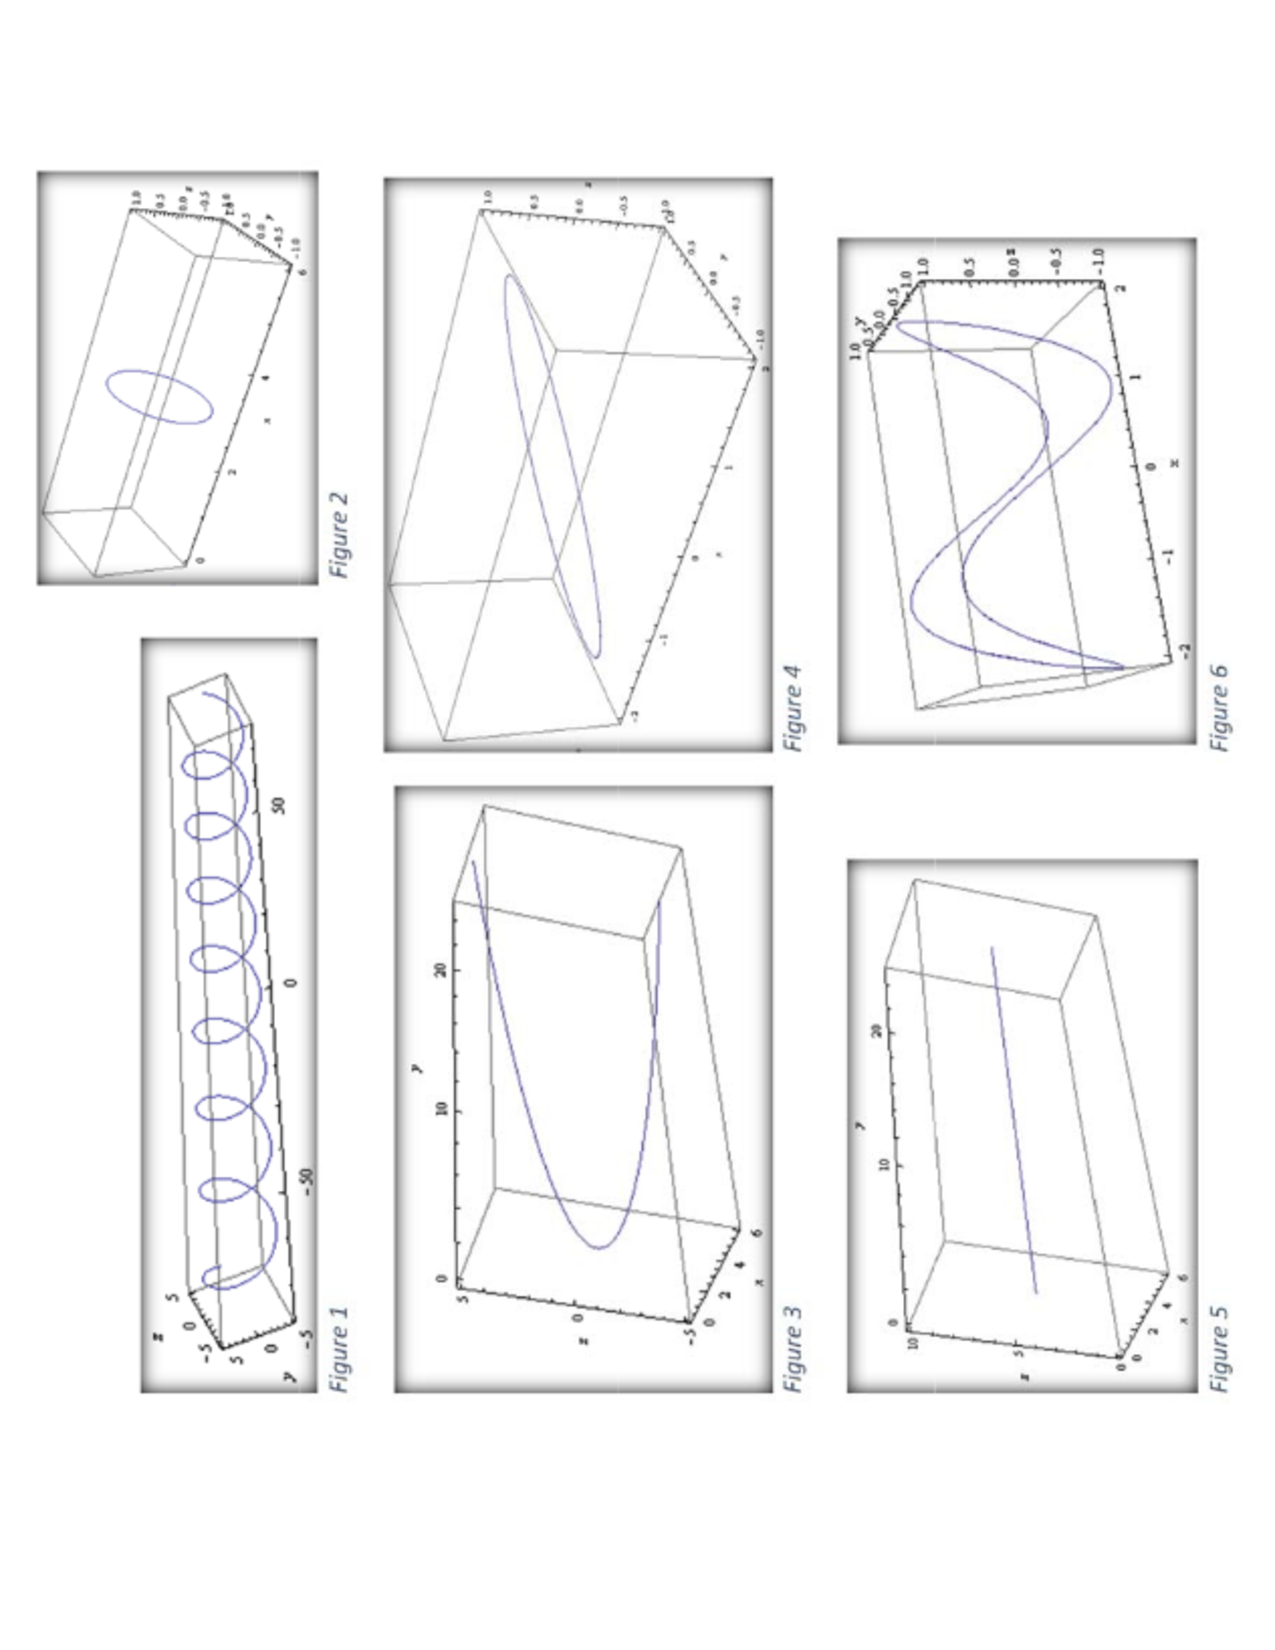
\includegraphics[angle=-89.99,trim= 40 120 0 120, scale=0.65]{Figure12-5-1.pdf}
	\end{image}
	
	\begin{freeResponse}
	\begin{enumerate}
	\item  {\bf Figure 5}.  This is a line with both $x$ and $z$ held fixed.
	
	\item  {\bf Figure 3}.  This is a parabola parallel to the $yz$-plane at $x=3$. 
	
	\item  {\bf Figure 2}.  This is a circle of radius $1$ in the plane $x=3$.  
	
	\item  {\bf Figure 1}.  The $x$-component is linear, while the projection onto the $yz$-plane is a circle of radius $5$.  
	So this looks like a ``spring''.
	
	\item  {\bf Figure 4}.  This is a circle with radius $1$ when projected onto the $xy$-plane.
	
	\item  {\bf Figure 6}.  This one is tricky.  Maybe the best way to spot it is that it is an ellipse when projected onto the $xy$-plane, while the $z$-component varies between $-1$ and $1$.
	
	\end{enumerate}
	\end{freeResponse}

\end{problem}

\begin{instructorNotes}

\end{instructorNotes}
















	
	
	
	
	
	
	
	
	

	










								
				
				
	














\end{document} 


















